\documentclass[]{beamer}
% Class options include: notes, notesonly, handout, trans,
%                        hidesubsections, shadesubsections,
%                        inrow, blue, red, grey, brown

% Theme for beamer presentation.
\usepackage{beamerthemesplit} 


\usepackage{multimedia}
\usepackage{hyperref}

\usepackage{collectbox}
\usepackage{amsmath}

\usepackage[utf8]{inputenc}
\usepackage[english]{babel}



%%%%%%%%%%%%%%%%%%%%%%%%%%%%%%%%%%%%%%%%%%%%%%%%%%%%%%%%%%%%%%%%%%%%%%



\definecolor{mypink1}{rgb}{0.858, 0.188, 0.478}

\definecolor{mygreen}{rgb}{0, 0.780, 0.494}
\definecolor{myorange}{rgb}{1., 0.557, 0}
\definecolor{myblue}{rgb}{0, 0.843, 1.}
\definecolor{mypink2}{rgb}{0.784, 0.416, 1.}

%%%%%%%%%%%%%%%%%%%%%%%%%%%%%%%%%%%%%%%%%%%%%%%%%%%%%%%%%%%%%%%%%%%%%%
% Other themes include: beamerthemebars, beamerthemelined, 
%                       beamerthemetree, beamerthemetreebars  

\title{PHY250: Review and Introduction}    % Enter your title between curly braces
\author{Anabela R. Turlione}                 % Enter your name between curly braces
\institute{Digipen Institute}      % Enter your institute name between curly braces
\date{Bilbao, Fall 2021}                    % Enter the date or \today between curly braces


\begin{document}

% Creates title page of slide show using above information
\begin{frame}
  \titlepage
\end{frame}
%\note{Talk for 30 minutes} % Add notes to yourself that will be displayed when
                           % typeset with the notes or notesonly class options

\section[]{}

% Creates table of contents slide incorporating
% all \section and \subsection commands
\begin{frame}
  \tableofcontents
\end{frame}

%%%%%%%%%%%%%%%%%%%%%%%%%%%%%%%%%%%%%%%%%%%%%%%%%%%%%%%%%%%%%%%%%%%
\section{Introduction}
\subsection{Review of PHY200}

\begin{frame}

  Until now, you have been describing the motion of a particle, using the equations of Newton:
\pause
\vspace{5mm}
\begin{equation}
  \sum_i\vec{F}_i=m\vec{a}
\end{equation}


\end{frame}

%%%%%%%%%%%%%%%%%%%%%%%%%%%%%%%%%%%%%%%%%%%%%%%%%%%%%%%%%%%%%%%%%%%




\begin{frame}

Then, you have defined the work done by a force,

\begin{equation}
  W=\int^2_1\vec{F}\cdot \vec{d\ell}
\end{equation}

\pause

And you have proved that:

\begin{equation}
  W=\Delta E_k
\end{equation}
\pause

Where

\begin{equation}
  E_k=\frac{1}{2}mv^2
\end{equation}

is the kinetic energy.
\end{frame}

%%%%%%%%%%%%%%%%%%%%%%%%%%%%%%%%%%%%%%%%%%%%%%%%%%%%%%%%%%%%%%%%%%%

\begin{frame}

 And, there are some kind of forces that have the following property: 

 \begin{equation}
  \oint\vec{F}\cdot \vec{d\ell}=0
\end{equation}

\pause
In this case, we can define the potential energy, and we say that the force is \textbf{conservative}


\begin{equation}
  \Delta U(\vec{r})=-\int^{\vec{r}}_{\vec{r}_0}\vec{F}\cdot \vec{d\ell}\pause \rightarrow \Delta U=W
\end{equation}

\pause

In this case, the total energy of the system is conserved:
\pause

\begin{equation}
 E=U+K=constant
\end{equation}

\end{frame}
  

%%%%%%%%%%%%%%%%%%%%%%%%%%%%%%%%%%%%%%%%%%%%%%%%%%%%%%%%%%%%%%%%%%%

\begin{frame}

So, when a force is conservative, that is, there is a function $U(x)$ such that

\begin{equation}
  F=-\frac{U(x)}{dx}
\end{equation}
 
then, the energy of the particle is constant. 


 \end{frame}
   
%%%%%%%%%%%%%%%%%%%%%%%%%%%%%%%%%%%%%%%%%%%%%%%%%%%%%%%%%%%%%%%%%%%

\begin{frame}

You also studied systems of $N$ particles,: 




  \begin{figure}[h!]
    \begin{center}
      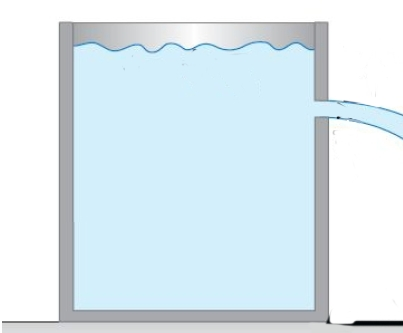
\includegraphics[height=2.in]{images/1.jpg}
    \end{center}
  \end{figure}

  







 \end{frame}

 
%%%%%%%%%%%%%%%%%%%%%%%%%%%%%%%%%%%%%%%%%%%%%%%%%%%%%%%%%%%%%%%%%%%

\begin{frame}

 And you defined the following vector quantities: 
  

  
    \pause
  
    \begin{equation}
      \vec{p}_i=m_i\vec{v}_i \pause ~ \textcolor{mypink1}{\rightarrow \vec{P}=\sum^N_i \vec{p}_i~~~(Linear~Momentum)}
    \end{equation}
    \pause
    \begin{equation}
      \vec{L}_i=\vec{r}_i\times\vec{p}_i ~ \pause \textcolor{mypink1}{\rightarrow \vec{L}=\sum^N_i \vec{L}_i~~~(Angular~Momentum)}
    \end{equation}
    \pause
    \begin{equation}
      \vec{\tau}_i=\vec{r}_i\times\vec{F}_i ~ \pause \textcolor{mypink1}{\rightarrow \vec{\tau}=\sum^N_i \vec{\tau}_i~~~(Torque)}
    \end{equation}

  
  
  
  
  
   \end{frame}


%%%%%%%%%%%%%%%%%%%%%%%%%%%%%%%%%%%%%%%%%%%%%%%%%%%%%%%%%%%%%%%%%%%
  \begin{frame}

    And found some interesting relations:
     
     \pause
     
     \begin{equation}
       \frac{\vec{dP}}{dt}=\vec{F}~\pause \textcolor{mypink1}{(Conservation~of~Linear~Momentum)}
     \end{equation}
     \pause
     \begin{equation}
       \frac{\vec{dL}}{dt}=\vec{\tau}~\pause \textcolor{mypink1}{(Conservation~of~Angular~Momentum)}
     \end{equation}
 
     
\end{frame}

      
%%%%%%%%%%%%%%%%%%%%%%%%%%%%%%%%%%%%%%%%%%%%%%%%%%%%%%%%%%%%%%%%%%%
\begin{frame}

  Finally, you have defined the center of mass of the system:
  \pause

  \begin{equation}
    \vec{R}_{CM}=\frac{1}{M}\sum^N_i=m_i\vec{r}_i
  \end{equation}

    \pause

  And you found the following expressions that relates the motion of the center of mass with the total external force:
  
  
  \begin{equation}
    \vec{P}=M\frac{d}{dt}(\vec{R}_{CM})=M\vec{V_{CM}}
  \end{equation}
  
   
  \begin{equation}
    \vec{F}^{ext}=M\frac{d^2}{dt^2}(\vec{R}_{CM})=M\vec{a_{CM}}
  \end{equation}

  \pause 
\vspace{3mm}

  So the center of mass moves as a particle acted by the total external force.

\end{frame}




%%%%%%%%%%%%%%%%%%%%%%%%%%%%%%%%%%%%%%%%%%%%%%%%%%%%%%%%%%%%%%%%%%%
\begin{frame}

In particular, for rotations of \textbf{ Rigid bodies} (the distances between particles are constant) in 2D:

\pause

\begin{equation}
 \vec{L}=I\vec{\omega }
\end{equation}

\begin{equation}
  \vec{\tau}= I\vec{\alpha }
 \end{equation}
  
 \pause
 where $\textbf{I}$ is the \textbf{Moment of Inertia }

 \begin{equation}
I=\sum^N_i m_i r^2_i
 \end{equation}
  
\end{frame}

%%%%%%%%%%%%%%%%%%%%%%%%%%%%%%%%%%%%%%%%%%%%%%%%%%%%%%%%%%%%%%%%%%%
\begin{frame}

  The total kinetic energy is:
  
  \pause
  \vspace{3mm}
  
  \begin{equation}
    E_k=\sum^N_i E_{k,i} \pause=\underbrace{\frac{1}{2}MV^2_{CM}}_{\textcolor{mypink1}{Translational~E_k}}+\underbrace{\frac{1}{2}\textit{I}\omega^2}_{\textcolor{mypink1}{Rotational~E_k}}
  \end{equation}
  
  \pause
  \vspace{3mm}
  
  Then, the motion of a system can be decomposed in:
  
  \pause 
  \begin{equation*}
    Tanslation~of~CM~+~Rotation~Around~CM
  \end{equation*}
  
  
  \end{frame}
%%%%%%%%%%%%%%%%%%%%%%%%%%%%%%%%%%%%%%%%%%%%%%%%%%%%%%%%%%%%%%%%%%%
\begin{frame}

  We can make a parallelism between the equations for cartesian coordinates and the equations for angular coordinates:

  
  \pause
  
  \begin{equation}
\vec{P}=M\vec{V}_{CM} \pause \leftrightarrow \vec{L}=I\vec{\omega }
  \end{equation}

  \pause
  
  \begin{equation}
\vec{F}=M\vec{a}_{CM}\pause \leftrightarrow \vec{\tau}=I\vec{\alpha }
  \end{equation}


  \end{frame}
  %%%%%%%%%%%%%%%%%%%%%%%%%%%%%%%%%%%%%%%%%%%%%%%%%%%%%%%%%%%%%%%%%%%
\begin{frame}

Finally, for continuous bodies, all the sums turns into integrals
  


\begin{equation}
  \vec{R}_{CM}=\frac{1}{M}\sum^N_i m_i \vec{r}_i \pause \rightarrow \int_V \rho(r) \vec{r} dv
\end{equation}

  \pause

\begin{equation}
    I=\sum^N_i m_i r^2_i \pause \rightarrow \int_V \rho(r) r^2 dv
\end{equation}


\pause



  \end{frame}
  %%%%%%%%%%%%%%%%%%%%%%%%%%%%%%%%%%%%%%%%%%%%%%%%%%%%%%%%%%%%%%%%%%%
  \subsection{PHY250}
\begin{frame}
In PHY250 we are going to extend the study of systems:

\vspace{5mm}

\pause
\begin{itemize}
  \item this time, the distance between their particles  may vary
  \pause
  \item we are going to study how the energy is propagated 
  \pause
  \item and we are going to study the thermal properties of matter
  \pause 
  \item finally, we are going to study the nature of light and how it interacts with different mediums 
\end{itemize}



    
    
    
\end{frame}
  
      

%%%%%%%%%%%%%%%%%%%%%%%%%%%%%%%%%%%%%%%%%%%%%%%%%%%%%%%%%%%%%%%
 \end{document}
%%%%%%%%%%%%%%%%%%%%%%%%%%%%%%%%%%%%%%%%%%%%%%%%%%%%%%%%%%%%%%%